
\documentclass[ucs]{beamer}

\usetheme{GSyC}
%\usebackgroundtemplate{\includegraphics[width=\paperwidth]{gsyc-bg.png}}


\usepackage[greek,spanish]{babel}   %greek permite usar euro 
\usepackage[utf8x]{inputenc}
\usepackage{graphicx}
\usepackage{amssymb} % Simbolos matematicos


% Metadatos del PDF, por defecto en blanco, pdftitle no parece funcionar
   \hypersetup{%
     pdftitle={json},%
     %pdfsubject={Diseño y Administración de Sistemas y Redes},%
     pdfauthor={GSyC},%
     pdfkeywords={},%
   }
%


% Para colocar un logo en la esquina inferior de todas las transpas
%   \pgfdeclareimage[height=0.5cm]{gsyc-logo}{gsyc}
%   \logo{\pgfuseimage{gsyc-logo}}


% Para colocar antes de cada sección una página de recuerdo de índice
%\AtBeginSection[]{
%  \begin{frame}<beamer>{Contenidos}
%    \tableofcontents[currentframetitle]
%  \end{frame}
%}



\begin{document}

% Entre corchetes como argumento opcional un título o autor abreviado
% para los pies de transpa
\title[json]{json }
%\subtitle{Diseño y Administración de Sistemas y Redes}
\author[GSyC]{Escuela Técnica Superior de Ingeniería de Telecomunicación\\
Universidad Rey Juan Carlos}
\institute{gsyc-profes (arroba) gsyc.urjc.es}
\date[2016]{Marzo de 2016}


%% TÍTULO
\begin{frame}
  \titlepage
  % Oportunidad para poner otro logo si se usó la opción nologo
  % \includegraphics[width=2cm]{logoesp}  
\end{frame}



%% LICENCIA DE REDISTRIBUCIÓN DE LAS TRANSPAS
%% Nota: la opción b al frame le dice que justifique el texto
%% abajo (por defecto c: centrado)
\begin{frame}[b]
\begin{flushright}
{\tiny
\copyright \insertshortdate~\insertshortauthor \\
  Algunos derechos reservados. \\
  Este trabajo se distribuye bajo la licencia \\
  Creative Commons Attribution Share-Alike 4.0\\
}
\end{flushright}  
\end{frame}



%% ÍNDICE
%\begin{frame}
%  \frametitle{Contenidos}
%  \tableofcontents
%\end{frame}



%the practice of system and network administration
%t limoncelli

%principles of network and system administration
%m burgess


\section{json}


%%---------------------------------------------------------------
\begin{frame}[fragile]
\frametitle{JSON}
Es un formato ligero para intercambiar datos, independiente del lenguaje de 
programación y de la plataforma
\begin{itemize}
\item
Estándar abierto, RFC 4627, año 2006
\item
Originalmente se consideraba subconjunto del lenguaje JavaScript y se
denominaba  \emph{JavaScript Object Notation}, aunque ya no es parte de JavaScript
\item
Diseñado como alternativa a XML, más ligero. Actualmente es más popular que XML
\item
Carece de algunas características de XML, por ejemplo gramáticas o diferencia entre texto y metadato 
\end{itemize}

\end{frame}

%%---------------------------------------------------------------
\begin{frame}[fragile]
\frametitle{Value}
\begin{center}
  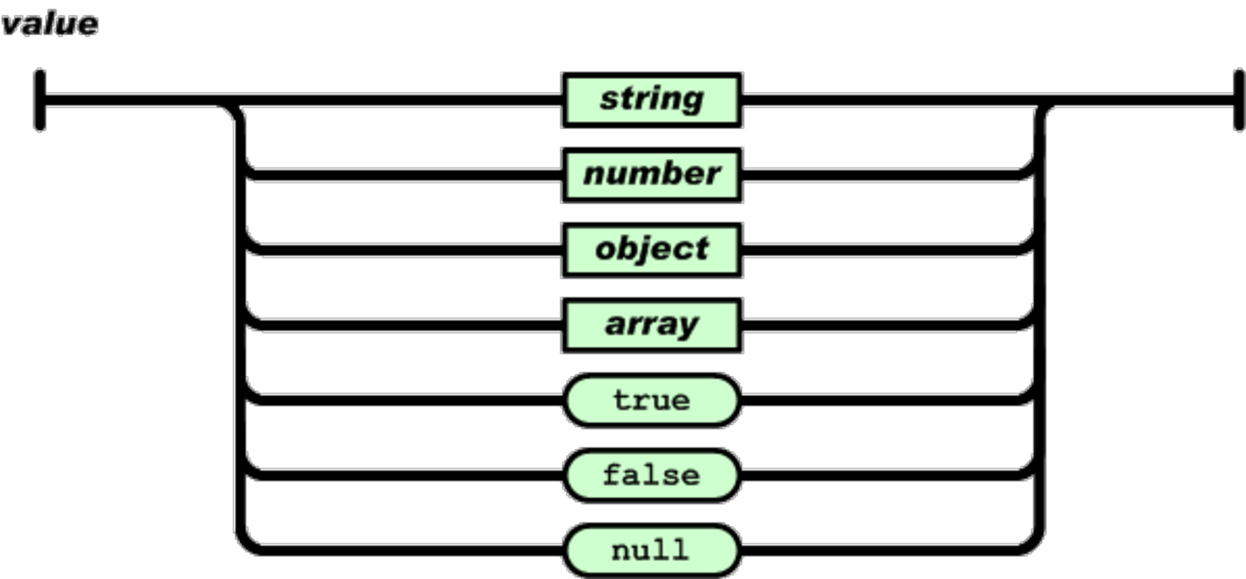
\includegraphics[width=09.0cm]{figs/value}
\end{center}
\begin{flushright}
\begin{tiny}
Fuente:json.org
\end{tiny}
\end{flushright}
\begin{itemize}
\item 
Un valor json puede ser un número, una cadena, un array o
un objeto, además de las constantes 
\emph{true},
\emph{false} y 
\emph{null}
\item
En python, las constantes equivalentes son 
\emph{True},
\emph{False} y 
\emph{None}
\end{itemize}
\end{frame}



%%---------------------------------------------------------------

\begin{frame}[fragile]
\frametitle{Number}
\begin{center}
  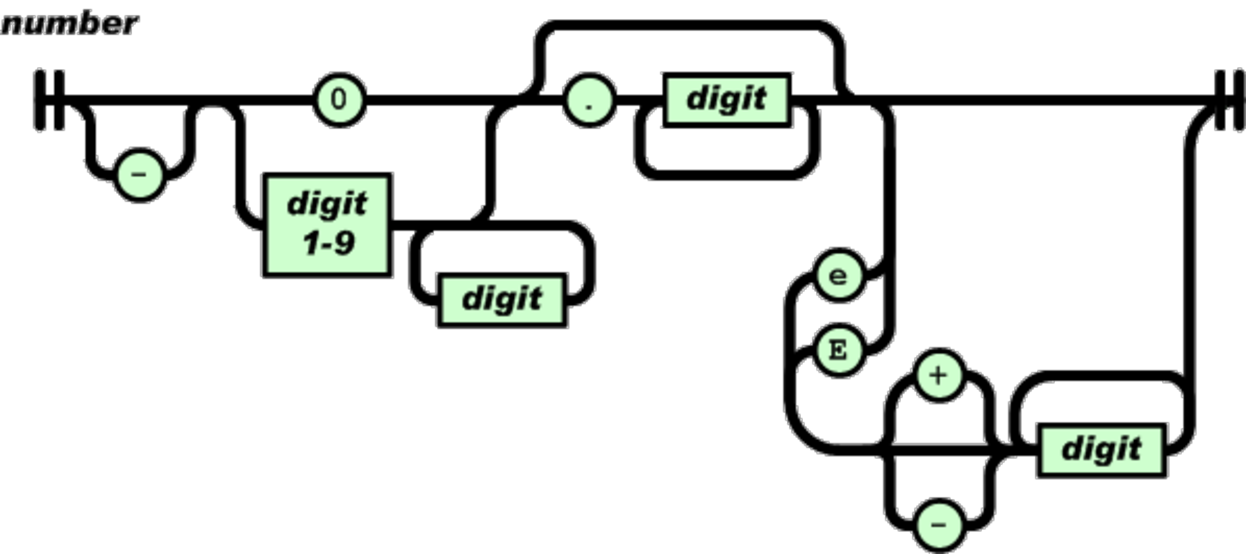
\includegraphics[width=08.5cm]{figs/number}
\end{center}
\begin{flushright}
\begin{tiny}
Fuente:json.org
\end{tiny}
\end{flushright}
\begin{itemize}
\item 
Los números son como las constantes numéricas
de cualquier lenguaje de programación moderno
\end{itemize}
\end{frame}

%%---------------------------------------------------------------

\begin{frame}[fragile]
\frametitle{String}
\begin{center}
  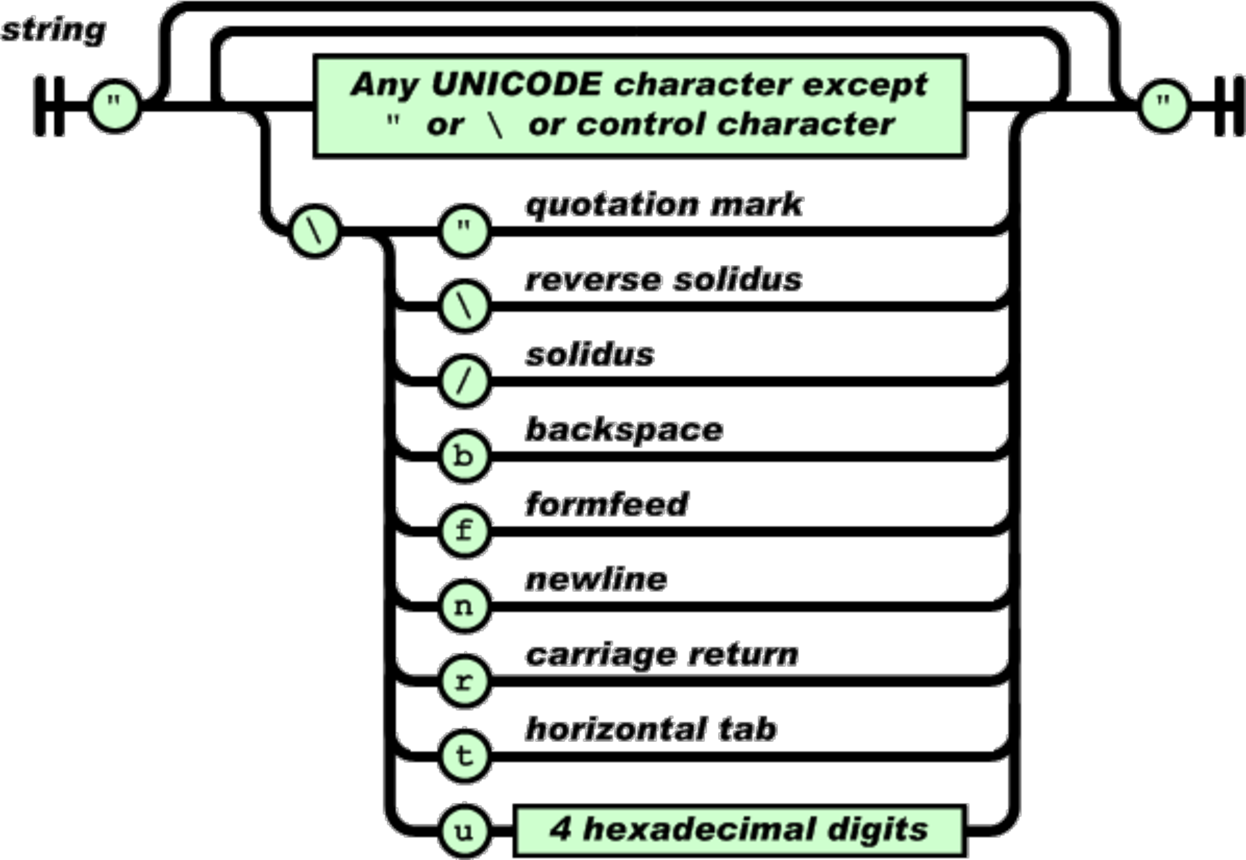
\includegraphics[width=07.0cm]{figs/string}
\end{center}
\begin{flushright}
\begin{tiny}
Fuente:json.org
\end{tiny}
\end{flushright}
\begin{itemize}
\item 
Las cadenas son como las de cualquier lenguaje de programación moderno
\item
A diferencia de python, el delimitador es únicamente la comilla doble,
no la comilla simple
\end{itemize}
\end{frame}

%%---------------------------------------------------------------
\begin{frame}[fragile]
\frametitle{Array}
\begin{center}
  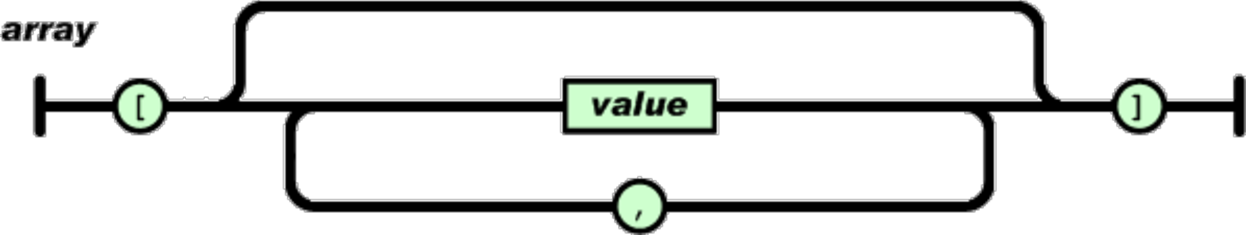
\includegraphics[width=10.5cm]{figs/array}
\end{center}
\begin{flushright}
\begin{tiny}
Fuente:json.org
\end{tiny}
\end{flushright}
\begin{itemize}
\item 
Un array es una secuencia de valores, separados por comas
\item
Como las listas de python
 
\end{itemize}
\end{frame}

%%---------------------------------------------------------------
\begin{frame}[fragile]
\frametitle{Objetos}
\begin{center}
  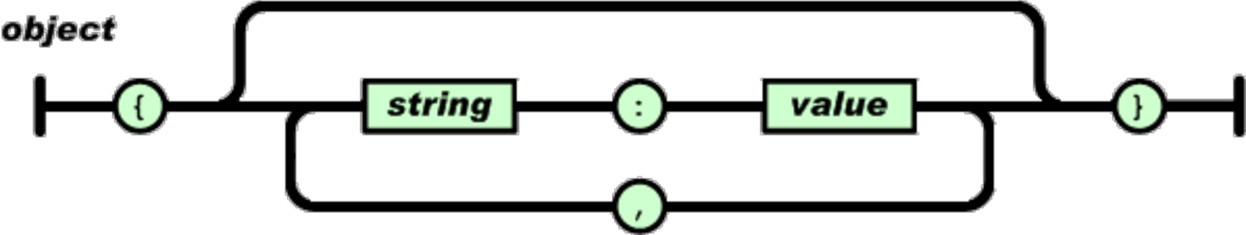
\includegraphics[width=10.5cm]{figs/object}
\end{center}
\begin{flushright}
\begin{tiny}
Fuente:json.org
\end{tiny}
\end{flushright}
\begin{itemize}
\item 
Un objeto es una secuencia de pares clave-valor, separados por comas
\item
Muy similar a los diccionarios de python, excepto porque

\begin{itemize}
\item
En python las claves pueden ser cadenas, números o tuplas
\item
En json las claves han de ser cadenas
\end{itemize}
 
\end{itemize}
\end{frame}


%%---------------------------------------------------------------
\begin{frame}[fragile]
\frametitle{Ejemplos correctos}
\begin{itemize}
\item
  \begin{footnotesize}
  \begin{verbatim}
"hola, mundo"
  \end{verbatim}
  \end{footnotesize}

\item

  \begin{footnotesize}
  \begin{verbatim}
4243.12
  \end{verbatim}
  \end{footnotesize}

\item
  \begin{footnotesize}
  \begin{verbatim}
-947e-5
  \end{verbatim}
  \end{footnotesize}

\item
  \begin{footnotesize}
  \begin{verbatim}
null
  \end{verbatim}
  \end{footnotesize}


\item
  \begin{footnotesize}
  \begin{verbatim}
[1,2,3,4]
  \end{verbatim}
  \end{footnotesize}


\end{itemize}
\end{frame}
%%----------------------------------------------
\begin{frame}[fragile]
\frametitle{}
\begin{itemize}

\item

  \begin{footnotesize}
  \begin{verbatim}
[1, "azul", [1,2,3]]
  \end{verbatim}
  \end{footnotesize}



\item
  \begin{footnotesize}
  \begin{verbatim}
[
    1, 
    "azul", 
    [
        1, 
        2, 
        3
    ]
]
  \end{verbatim}
  \end{footnotesize}



\item
  \begin{footnotesize}
  \begin{verbatim}
["as" ,   "dos", "tres"]
  \end{verbatim}
  \end{footnotesize}


\item
  \begin{footnotesize}
  \begin{verbatim}
["sota", "caballo", "rey"]
  \end{verbatim}
  \end{footnotesize}

\item
  \begin{footnotesize}
  \begin{verbatim}
[
    "sota",
    "caballo",
    "rey"
]
  \end{verbatim}
  \end{footnotesize}

\end{itemize}

\end{frame}



%%---------------------------------------------------------------
\begin{frame}[fragile]
\frametitle{}
\begin{itemize}




\item
  \begin{footnotesize}
  \begin{verbatim}
{ "nombre":"Juan", "apellido":"Pérez"}
  \end{verbatim}
  \end{footnotesize}
\item
  \begin{footnotesize}
  \begin{verbatim}
{ "v1":true, "v2":null, "v3":false}
  \end{verbatim}
  \end{footnotesize}
\item
  \begin{footnotesize}
  \begin{verbatim}
{ "nombre": "Juan", "notas":[5.5, 7.2, 6.1]}
  \end{verbatim}
  \end{footnotesize}
\item
  \begin{footnotesize}
  \begin{verbatim}
{
    "nombre": "Juan", 
    "notas": [
        5.5, 
        7.2, 
        6.1
    ]
}
  \end{verbatim}
  \end{footnotesize}
\end{itemize}

\end{frame}


%%---------------------------------------------------------------
\begin{frame}[fragile]
\frametitle{Ejemplos incorrectos}
\begin{itemize}
\item
  \begin{footnotesize}
  \begin{verbatim}
True
  \end{verbatim}
  \end{footnotesize}

\item

  \begin{footnotesize}
  \begin{verbatim}
'hola, mundo'
  \end{verbatim}
  \end{footnotesize}

\item
  \begin{footnotesize}
  \begin{verbatim}
{"hola,mundo"}
  \end{verbatim}
  \end{footnotesize}

\item
  \begin{footnotesize}
  \begin{verbatim}
{1:"uno", 2:"dos"}
  \end{verbatim}
  \end{footnotesize}
\end{itemize}

\end{frame}



%%---------------------------------------------------------------
\begin{frame}[fragile]
\frametitle{Generación de json desde python}
A partir de un objeto python, es muy sencillo generar un valor json
\begin{itemize}
\item
\verb|json.dumps()| recibe un objeto python, devuelve una cadena con el valor equivalente en json
\end{itemize}

  \begin{footnotesize}
  \begin{verbatim}
>>> import json
>>> json.dumps(2.23)
'2.23'
>>> json.dumps('Hola,mundo')
'"Hola,mundo"'
>>> json.dumps(True)
'true'
>>> json.dumps(None)
'null'
>>> json.dumps([1,2,3])
'[1, 2, 3]'
>>> json.dumps({1:"uno",2:"dos"})
'{"1": "uno", "2": "dos"}'
  \end{verbatim}
  \end{footnotesize}
\end{frame}



%%---------------------------------------------------------------
\begin{frame}[fragile]
\frametitle{}
\verb|json.dumps()| admite parámetros adicionales
\begin{itemize}
\item
\verb|sort_keys=True| 

ordena las claves por orden alfabético
\item
\verb|indent=4| 

hace \emph{pretty printing}, tabulando con el número de espacios indicado (4 en el ejemplo)
\item
\verb|sort_keys=True| 

ordena las claves alfabéticamente
\end{itemize}

  \begin{footnotesize}
  \begin{verbatim}
>>> print json.dumps({"nombre":"Juan","apellido":"Blanco"}, 
    sort_keys=True, indent=4)
{
    "apellido": "Blanco",
    "nombre": "Juan"
}
  \end{verbatim}
  \end{footnotesize}

\end{frame}


%%---------------------------------------------------------------
\begin{frame}[fragile]
\frametitle{Decodificación de json desde python}
Es muy sencillo leer valores json desde python
\begin{itemize}
\item
\verb|json.loads()| recibe una cadena con un valor json, devuelve un objeto python
\end{itemize}

  \begin{footnotesize}
  \begin{verbatim}
>>> print json.loads('9.5')
9.5
>>> print json.loads('[1,2,3]')
[1, 2, 3]
>>> print json.loads('null')
None
  \end{verbatim}
  \end{footnotesize}
\end{frame}


%%---------------------------------------------------------------
\begin{frame}[fragile]
\frametitle{}
\begin{itemize}
\item
\verb|json.loads()| recibe una cadena con el valor json. Si el valor es a su
vez una cadena, tendremos una cadena dentro de una cadena
\item
Como el delimitador de cadena en json es la comilla doble, en python es recomendable
emplear como delimitador la comilla simple (es más legible que escapar la comilla doble)
\end{itemize}

  \begin{footnotesize}
  \begin{verbatim}
>>> print json.loads('"Hola,mundo"')
Hola,mundo
>>> print json.loads('{"nombre":"Juan","apellido":"Blanco"}')
{u'nombre': u'Juan', u'apellido': u'Blanco'}
  \end{verbatim}
  \end{footnotesize}

\end{frame}


%%---------------------------------------------------------------
\begin{frame}[fragile]
\frametitle{Otras librerías}
Además de la implementación de la librería estándar de python,
hay otras librerías para codificar y decodificar json, con la misma API, diseñadas para ofrecer mejor
rendimiento en situaciones especiales
\begin{itemize}
\item
simplejson
\item
pyson
\item
Yajl-Py
\item
ultrajson
\item
metamagic.json
\end{itemize}

\end{frame}





\end{document}

